%=====================================================================
% manuscript_main.tex
% Target journal: Stochastic Environmental Research and Risk Assessment (SERRA)
% Springer Nature LaTeX template: sn-jnl, two-column iicol layout
% Compile: pdflatex -> bibtex -> pdflatex -> pdflatex
%=====================================================================

\documentclass[pdflatex,sn-basic,iicol]{sn-jnl}

%---------------------------------------------------------------------
% Packages
%---------------------------------------------------------------------

\usepackage[utf8]{inputenc}
\usepackage[T1]{fontenc}
\usepackage{lmodern}
\usepackage{amsmath,amssymb}
\usepackage{booktabs}
\usepackage{graphicx}
\usepackage{siunitx}
\usepackage{xcolor}
\usepackage{array}
\usepackage{multirow}
\usepackage{rotating}
\usepackage{enumitem}
\usepackage{pdflscape}
\usepackage{float}
\usepackage{placeins}
\usepackage{adjustbox}
\usepackage{lineno}
\usepackage{hyperref}

% The local sn-jnl class exposes \orcid{<URL>} but its optional logo asset
% is not included in this repository; retain the class hyperlink metadata.
\renewcommand{\orcidlogo}{}

\hypersetup{
  colorlinks=true,
  linkcolor=blue,
  citecolor=blue,
  urlcolor=blue,
  pdfborder={0 0 0}
}

%---------------------------------------------------------------------
% Macros
%---------------------------------------------------------------------

\newcommand{\PMten}{\ensuremath{\mathrm{PM}_{10}}}

% Layout tuning for the Springer Nature iicol two-column format.
\setlength{\tabcolsep}{4pt}
\renewcommand{\arraystretch}{1.08}
\setlength{\textfloatsep}{10pt plus 2pt minus 2pt}
\setlength{\floatsep}{8pt plus 2pt minus 2pt}
\setlength{\intextsep}{8pt plus 2pt minus 2pt}

%---------------------------------------------------------------------
% Title page
%---------------------------------------------------------------------

\title[Descriptive horizon gains vs global inferential support in \PMten{} forecasting]
{When descriptive forecast-horizon gains do not imply global evidence
of incremental meteorological predictability: a multi-site \PMten{} study}

% Author details for submission.
\author*[1]{\fnm{Federico} \sur{García Crespí}\orcid{https://orcid.org/0000-0002-7129-7791}}\email{fedeg@umh.es}
\affil*[1]{\orgdiv{Departamento de Ingeniería de Computadores},
  \orgname{Universidad Miguel Hernández de Elche},
  \orgaddress{\city{Elche}, \country{Spain}}}

\abstract{Forecast skill relative to persistence is often summarised by how long an
improvement lasts, but a longer skill horizon does not necessarily provide equally
strong evidence that an added information set contributes incremental predictive
information. We evaluate hourly \PMten{} forecasts at nine sites (Madrid Casa de
Campo and eight Irish stations) over January--July 2023 using an expanding-window
rolling-origin scheme with 24-h spacing between forecast origins and horizons
$h=1,\ldots,24$. The incremental comparison uses the same direct multi-horizon
XGBoost learner with two information sets: pollutant lags alone and pollutant lags
plus meteorological observations available at the forecast origin. This is an
observational information-set experiment, not an evaluation using future numerical
weather prediction (NWP) forecasts. In Madrid, adding meteorology extends the strict
longest-contiguous positive persistence-relative skill horizon from 9 to 17~h
(+8~h), whereas the relaxed last-positive-skill horizon increases from 15 to 17~h
(+2~h). However, none of the 36 dimensionally corrected comparisons using the
Diebold--Mariano test with Harvey--Leybourne--Newbold correction (DM-HLN) at
$h\in\{1,6,12,24\}$ survives global Bonferroni correction under either the
overlap-based specification ($q_{\text{overlap}}=0$; 0/36) or a fixed automatic
Newey--West sensitivity allowing positive-lag dependence (0/36). Thus, descriptive
horizon extension is evident at some sites, but family-wise global support for
attributing those gains to incremental meteorological information remains limited.}

\keywords{PM10, rolling-origin evaluation, persistence-relative skill, forecast horizon, Diebold--Mariano test, multiplicity}

\begin{document}

\maketitle
\linenumbers

\section{Introduction}
\label{sec:intro}
% ─────────────────────────────────────────────────────────────────────────────

The usefulness of an air-quality forecast depends strongly on lead time. A
model may improve near-term accuracy while offering little advantage later,
so an hourly \PMten{} forecast is useful only for as long as it remains better
than a simple persistence reference. Persistence is therefore not merely a
convenient baseline. It provides a demanding test of whether a forecasting
system adds information beyond the most recent observation in a setting where
concentrations reflect emissions together with meteorologically driven
transport and mixing \citep{Seinfeld2006, Kumar2016}.

That comparison becomes less straightforward when meteorological covariates
are added. Pollutant history already contains information about some of the
same underlying processes, so a reduction in forecast error after adding
meteorology may reflect genuinely incremental information, a different
representation of structure already present in lagged \PMten{}, or a mixture
of both. The balance can also change with site and lead time. Published
forecasting gains therefore span heterogeneous designs and outcomes
\citep{Mendez2023, Pak2018, Bai2018, AnsariQuaff2025}.

The central distinction is between a descriptive and an inferential claim. A
model may remain better than persistence over more horizons after meteorology
is added, making the extension descriptively meaningful. That observation
alone, however, does not establish how strongly the added information is
supported once sampling uncertainty and multiple comparisons are considered.

We examine this distinction in a nine-site hourly \PMten{} experiment
comprising Madrid Casa de Campo and eight Irish stations, evaluated over
January--July 2023 with an expanding-window rolling-origin design. Persistence
and SARIMA serve as reference benchmarks. The incremental comparison holds
the learner fixed and contrasts direct multi-horizon XGBoost based on
pollutant lags with the same model augmented by meteorological observations
available at the forecast origin. We summarise horizon-wise performance using
persistence-relative RMSE skill curves and the descriptive horizon measures
$H^*$, and assess inferential attribution with DM-HLN tests
\citep{Diebold1995, Harvey1997} at $h\in\{1,6,12,24\}$ under global
multiplicity control across the 36 planned site--horizon comparisons.

This design reveals an important separation between the two levels of
evidence. Some sites show sizeable descriptive extensions of
persistence-relative skill, yet these gains provide weak family-wise global
support for incremental meteorological predictability after accounting for
the planned inferential family. Allowing residual positive-lag dependence
through a fixed automatic Newey--West sensitivity leaves that global
conclusion unchanged, although the limited local signals depend more on the
specification.

\section{Data}
\label{sec:data}
% ─────────────────────────────────────────────────────────────────────────────

\subsection{Madrid}

Hourly \PMten{} concentrations and concurrent meteorological measurements were
obtained for Madrid Casa de Campo from the Madrid City Council open-data portal.
The station is classified as an urban-background site on the western edge of
the city, away from major point sources, and is representative of citywide
background conditions.  The study period spans January 2020 through July 2023;
records with missing \PMten{} or meteorological data were flagged and excluded
from model training and evaluation on a per-origin basis.  Seven meteorological
variables were retained: precipitation (\textit{rain}), temperature
(\textit{temp}), relative humidity (\textit{rhum}), mean sea-level pressure
(\textit{msl}), wind speed (\textit{wdsp}), wind direction (\textit{wddir}),
and solar radiation.

\subsection{Ireland}

Hourly \PMten{} concentrations and meteorological covariates were obtained from
the Irish Environmental Protection Agency (EPA) monitoring network.  Eight
stations distributed across Ireland were selected on the basis of data
completeness over the study window (January 2020 -- July 2023):
Birr (Co.\ Offaly), Dublin Airport, Dundalk (Co.\ Louth), Pearse Street
Dublin, Ringsend Dublin, Edenderry (Co.\ Offaly), Henry Street Limerick, and
Portlaoise (Co.\ Laois).  Meteorological variables were extracted from the nearest
mapped EPA synoptic station for each monitoring site.

Table~\ref{tab:descriptive} summarises the basic \PMten{} statistics for all
nine sites over the training and evaluation periods.  Concentrations are
generally low to moderate, with training-period means ranging from
11.3~\si{\micro\gram\per\cubic\metre} (Portlaoise) to
19.1~\si{\micro\gram\per\cubic\metre} (Dublin Airport), and Madrid at
18.4~\si{\micro\gram\per\cubic\metre}.  The training-period 95th percentile
exceeds 40~\si{\micro\gram\per\cubic\metre} at four of nine sites: Madrid,
Dublin Airport, Ringsend Dublin, and Edenderry.
Data completeness is high: missing rates are below 2\% at all
sites during both periods.

\begin{table*}[!t]
\centering
\caption{Descriptive statistics of hourly \PMten{}
  (\si{\micro\gram\per\cubic\metre}) for all nine sites.
  Training: 2020--2022; evaluation: Jan--Jul 2023.
  $n$: valid hourly observations; miss: missing rate (\%).}
\label{tab:descriptive}
\small
\begin{adjustbox}{max width=0.98\textwidth}
\begin{tabular}{lrrrrrrrr}
\toprule
 & \multicolumn{4}{c}{Training (2020--2022)} & \multicolumn{4}{c}{Evaluation (2023)} \\
\cmidrule(lr){2-5}\cmidrule(lr){6-9}
Station & $n$ & Mean & SD & P95 & $n$ & Mean & SD & P95 \\
\midrule
Madrid              & 25\,630 & 18.4 & 20.0 & 42.0 & 4\,988 & 15.9 & 12.3 & 34.6 \\
\midrule
Birr                & 20\,372 & 12.8 & 12.5 & 31.4 & 5\,085 & 13.2 & 11.3 & 31.2 \\
Dublin Airport      & 21\,958 & 19.1 & 16.1 & 46.9 & 3\,504 & 15.7 & 10.9 & 34.3 \\
Dundalk             & 21\,938 & 11.4 &  8.6 & 24.3 & 3\,658 & 13.1 & 10.2 & 30.7 \\
Pearse St.\ Dublin  & 17\,009 & 13.0 &  9.9 & 30.2 & 5\,088 & 15.4 & 10.1 & 33.3 \\
Ringsend Dublin     & 21\,949 & 15.6 & 16.1 & 41.9 & 5\,087 & 14.0 & 13.1 & 36.7 \\
Edenderry           & 11\,526 & 17.8 & 19.8 & 48.8 & 5\,029 & 15.9 & 16.0 & 38.5 \\
Henry St.\ Limerick & 13\,128 & 13.0 & 12.1 & 30.8 & 5\,052 & 11.9 &  8.6 & 27.2 \\
Portlaoise          & 21\,958 & 11.3 &  9.7 & 27.5 & 5\,088 & 10.9 &  7.9 & 25.1 \\
\bottomrule
\end{tabular}
\end{adjustbox}
\end{table*}

% ─────────────────────────────────────────────────────────────────────────────
\section{Methods}
\label{sec:methods}
% ─────────────────────────────────────────────────────────────────────────────

\subsection{Backtesting protocol}

We adopt a rolling-origin expanding-window backtesting scheme to preserve
prospective temporal information flow and strict separation between training
and evaluation data.  For each forecast origin $t$, the training window covers
all available observations up to (but not including) $t$; no future information
is used at any point.  The forecast origin advances in daily strides of 24~h,
producing one $h = 1, \ldots, 24$ forecast vector per day.

The evaluation period was 1 January--31 July 2023, with forecast origins spaced
by 24~h.  The number of valid evaluated origins varied by site according to data
availability.
The mandatory minimum training window is 8\,760 observations (one year), so
origins in early 2023 draw on three years of history.  This protocol prevents
look-ahead from future observations in the rolling-origin evaluation.  Model configurations and feature sets used in the
evaluation were held fixed across evaluation origins; no origin-level tuning or
cross-validation was performed.

\subsection{Model specifications}

\subsubsection{Persistence.}
The persistence model predicts $\hat{y}_{t+h} = y_t$ for all $h$.  It serves
as the denominator benchmark for the skill score.

\paragraph{SARIMA.}
We fit a SARIMA(1,0,1)(1,0,0)$_{24}$ model at each origin using the
\textit{statsmodels} implementation of exact maximum likelihood.  To avoid
numerical instability of the Kalman filter on very long training windows, the
training series is truncated to the most recent 17\,520 observations
(approximately two calendar years) at each origin.  Multi-step-ahead forecasts
are generated by iterating the fitted state-space model forward.  SARIMA is
treated as a univariate statistical reference; it does not receive
meteorological inputs.

\paragraph{XGBoost --- lags only.}
A separate XGBoost regressor \citep{Chen2016} is trained for each horizon
$h \in \{1, \ldots, 24\}$ (the \emph{direct} multi-horizon strategy).  The
feature set consists of eight lagged \PMten{} values
($y_{t-1}, y_{t-2}, y_{t-3}, y_{t-6}, y_{t-12}, y_{t-24}, y_{t-48},
y_{t-168}$) and four calendar indicators (hour of day, day of week, month,
Julian day).  Hyperparameters are fixed across all origins and horizons
(Table~\ref{tab:xgb_params}) to ensure fair comparison; no origin-level
cross-validation is performed.

\paragraph{XGBoost --- lags + meteorology.}
Identical to the lags-only model except that the meteorological variables
measured at time $t$ are appended to the feature vector (seven for Madrid, nine for the Irish stations).  This is an
\emph{observational} setup in which meteorological information is available at
the moment of forecast issuance.  Madrid uses concurrent station observations,
whereas the Irish covariates come from the nearest mapped EPA synoptic station.
Because observed meteorological values are used
rather than numerical weather prediction (NWP) forecasts, the reported skill
scores should not be interpreted as operational performance with NWP inputs (see Section~\ref{sec:discussion}).

\begin{table}[t]
\centering
\small
\caption{Fixed XGBoost hyperparameters used for all models and horizons.}
\label{tab:xgb_params}
\begin{tabular}{ll}
\toprule
Parameter & Value \\
\midrule
Number of estimators & 300 \\
Maximum tree depth & 4 \\
Learning rate & 0.05 \\
Row subsampling & 0.90 \\
Column subsampling & 0.90 \\
Objective & \texttt{reg:squarederror} \\
Random seed & 42 \\
\bottomrule
\end{tabular}
\end{table}

\subsection{Evaluation metrics}

\subsubsection{Skill score.}
For each model $m$ and horizon $h$, the RMSE skill score relative to
persistence is:
\begin{equation}
  S_m(h) = 1 - \frac{\mathrm{RMSE}_m(h)}{\mathrm{RMSE}_{\text{pers}}(h)},
  \label{eq:skill}
\end{equation}
where the RMSEs are computed over all forecast origins in the evaluation period.
The definition used throughout the skill-curve analysis is given in
Eq.~\ref{eq:skill}.
Positive $S_m(h)$ indicates that model $m$ outperforms persistence at horizon
$h$.

\paragraph{Useful forecast horizon \texorpdfstring{$H^*$}{H*}.}
We report two descriptive persistence-relative horizon summaries based on the sign of
$S_m(h)$ over $h\in\{1,\ldots,24\}$:
\begin{itemize}
  \item \textbf{$H^*_{\text{strict}}$ (primary)}: the length of the longest \emph{contiguous} run of horizons with $S_m(h)>0$.
  \item \textbf{$H^*_{\text{relax}}$ (secondary)}: the last horizon $h$ for which $S_m(h)>0$.
\end{itemize}
$H^*$ is a descriptor of the skill-curve sign pattern and is not itself a hypothesis
test.

\paragraph{Diebold--Mariano test (DM-HLN), dependence specification, and multiplicity.}
Incremental meteorological information is assessed inferentially via horizon-wise
Diebold--Mariano tests \citep{Diebold1995} with the Harvey--Leybourne--Newbold
finite-sample correction \citep{Harvey1997} (DM-HLN), comparing squared-error losses of
XGBoost (lags only) versus XGBoost (lags + meteorology) at physical horizons
$h\in\{1,6,12,24\}$.

Because forecasts are issued once per day (24-h origin spacing), the loss-differential
sequence advances in daily steps rather than in physical hours.  We therefore define
$h_{\text{DM}}=\lceil h/24\rceil$ as the horizon expressed in loss-differential steps.
For $h\in\{1,6,12,24\}$, $h_{\text{DM}}=1$ for all tests, so the mechanically induced
overlap bandwidth is $q_{\text{overlap}}=\max(0,h_{\text{DM}}-1)=0$.  This
overlap-based choice removes the \emph{mechanically required} positive-lag covariance
from overlapping multi-step forecast errors, but it does not imply that loss
differentials are independent or that residual dependence cannot exist.

To address potential positive-lag dependence not induced mechanically by overlap, we
also report a fixed automatic Newey--West sensitivity analysis \citep{NeweyWest1987}
using the bandwidth rule $q_{\text{auto}}=\lfloor 4\,(n/100)^{2/9}\rfloor$.

The primary inferential family comprises the 36 planned site--horizon comparisons
(9 sites $\times$ 4 horizons), controlled with global Bonferroni correction.  As a
within-station sensitivity analysis addressing a narrower inferential scope, we also
apply Benjamini--Hochberg false-discovery-rate control separately within each station
(4 horizons per station).

% ─────────────────────────────────────────────────────────────────────────────
\section{Results}
\label{sec:results}
% ─────────────────────────────────────────────────────────────────────────────

\subsection{Madrid---substantial descriptive horizon extension}

Madrid provides the clearest descriptive contrast between the two XGBoost
information sets. The lags-only model remains better than persistence over
only part of the 24-h range, whereas adding meteorological observations
extends positive persistence-relative skill further into the day
(Figure~\ref{fig:madrid_skill}). The primary strict descriptor captures the
largest change: the longest contiguous positive-skill run increases from
$H^*_{\text{strict}}=9$~h with lags only to
$H^*_{\text{strict}}=17$~h with lags + meteorology, an extension of +8~h.
The relaxed descriptor changes less, from 15 to 17~h (+2~h). These summaries
answer different descriptive questions. The strict measure reflects
continuity of positive skill, whereas the relaxed measure records the last
horizon for which $S(h)>0$. Reporting both therefore shows how the apparent
size of the horizon gain depends on the feature of the skill profile being
summarised.

\begin{figure*}[!t]
  \centering
  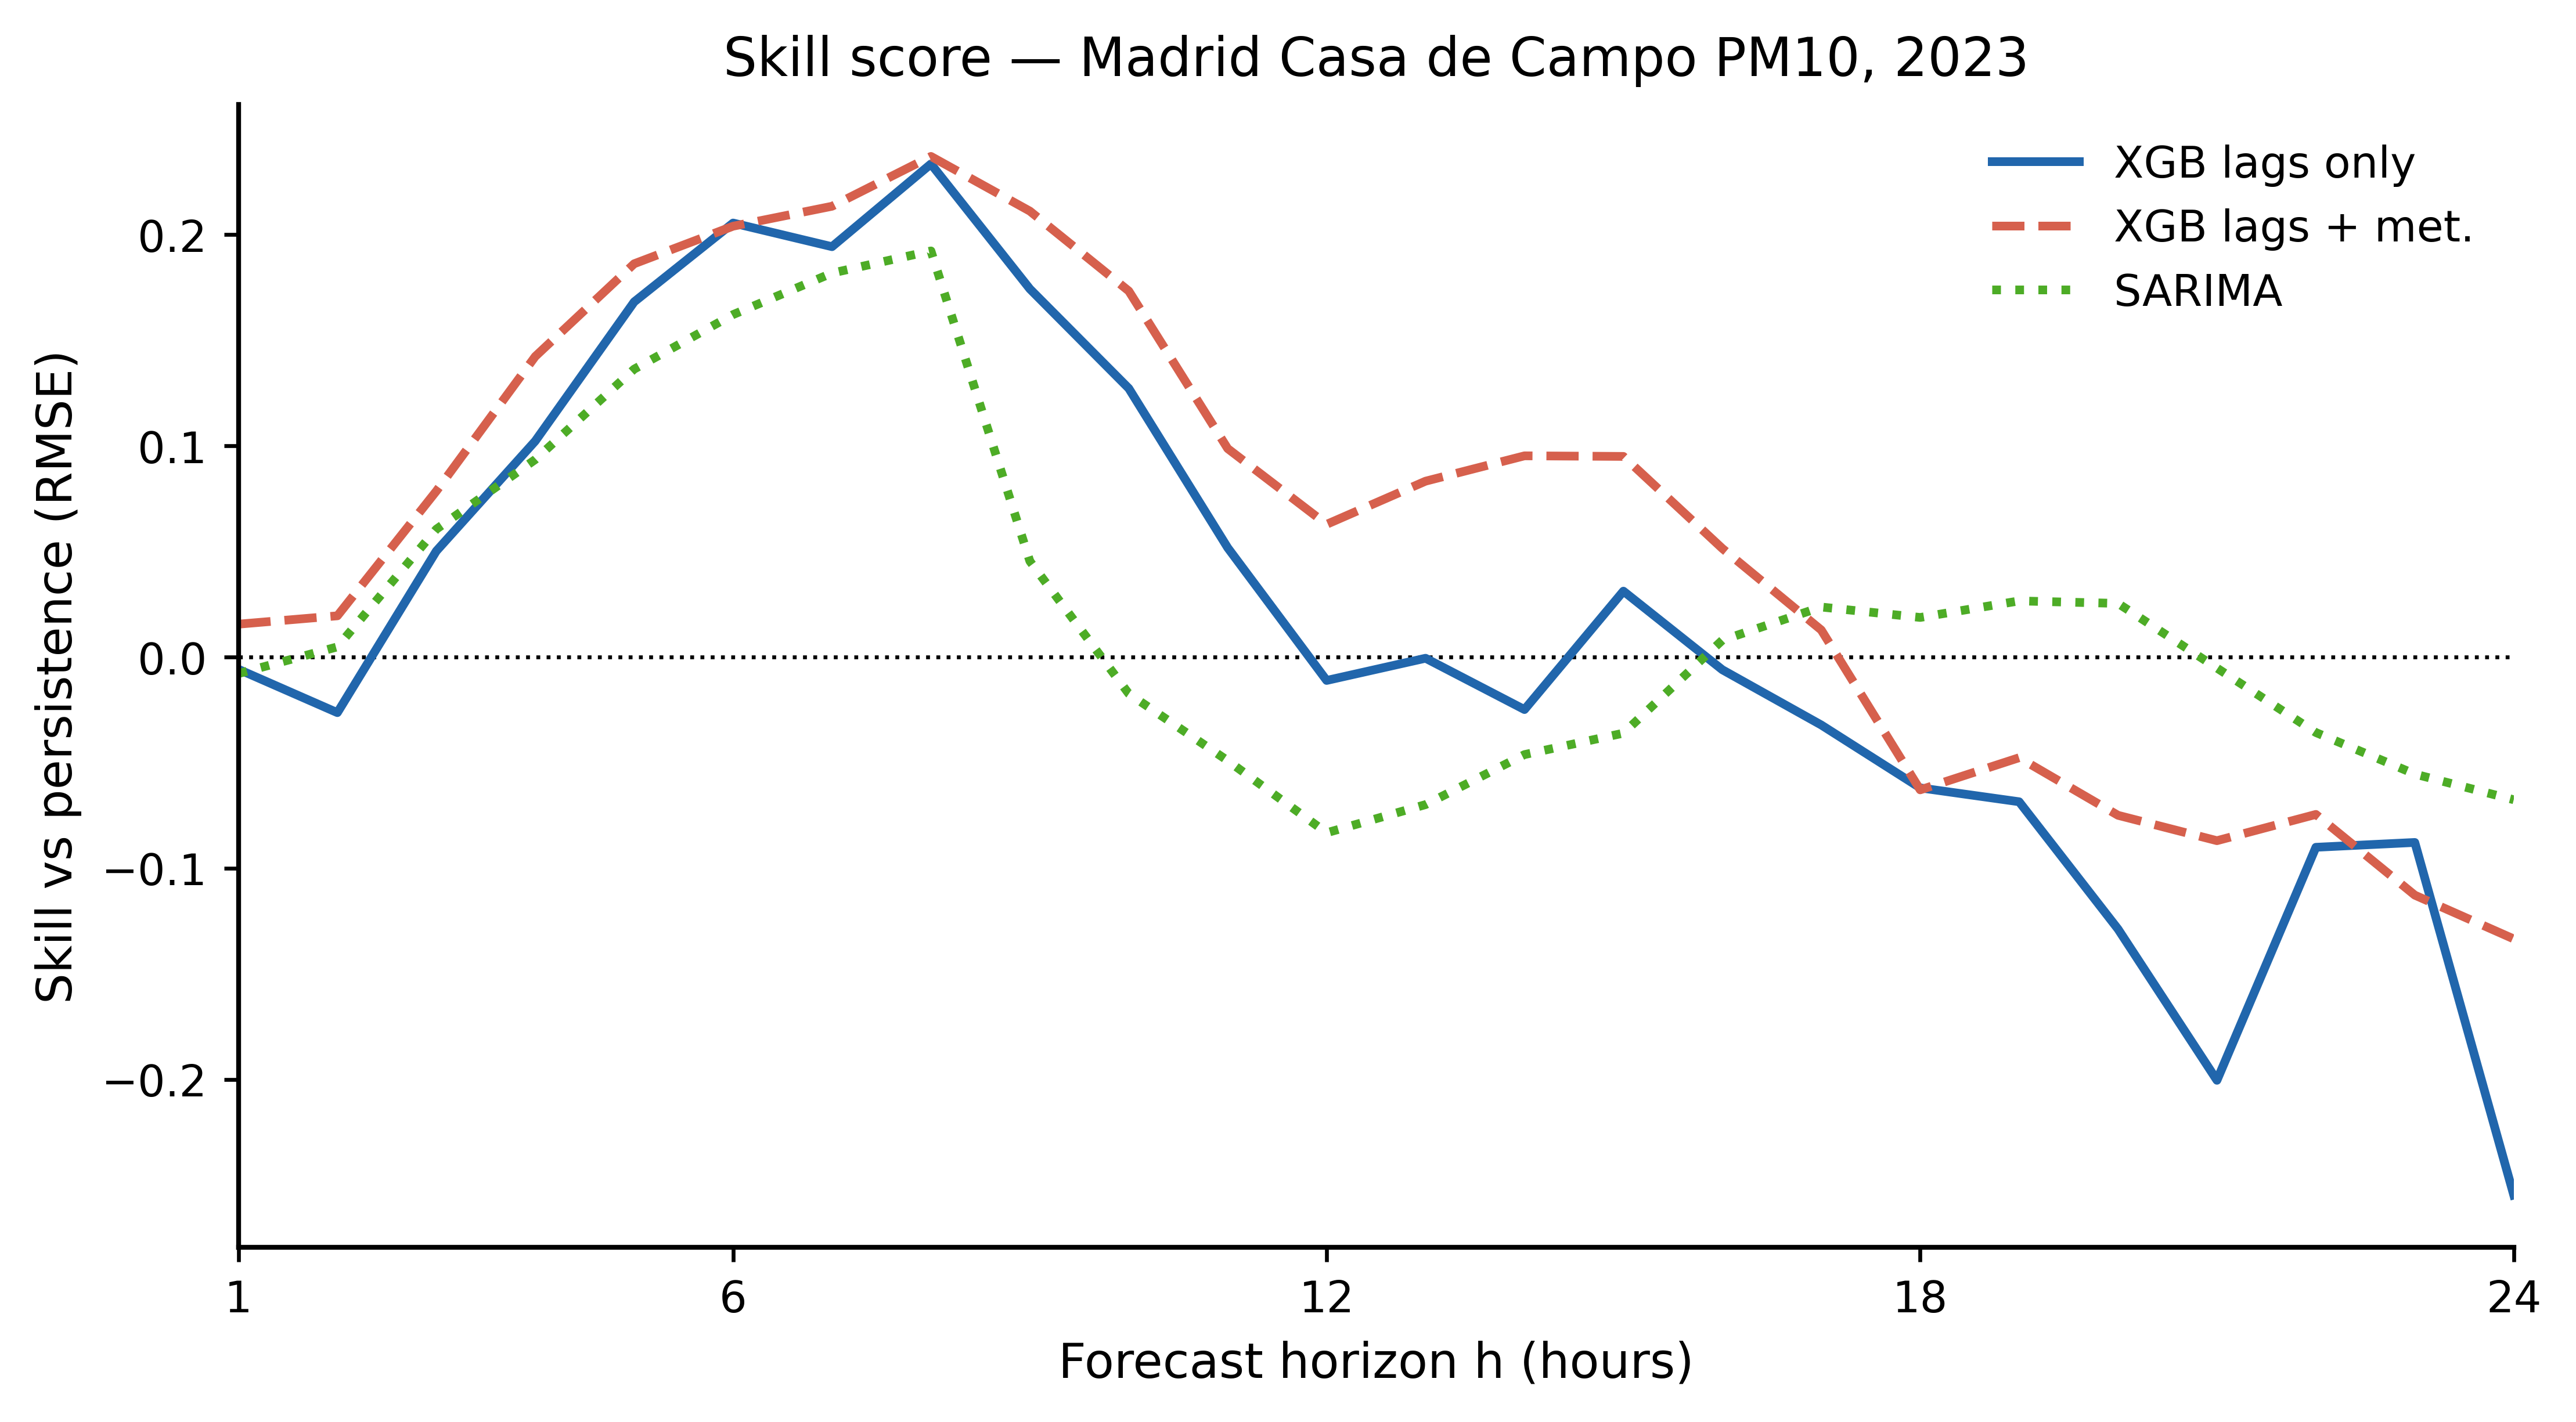
\includegraphics[width=0.92\textwidth]{serra_fig1_madrid_skill_curves.png}
  \caption{Madrid Casa de Campo (Jan--Jul 2023): persistence-relative RMSE skill
    $S_m(h)=1-\mathrm{RMSE}_m(h)/\mathrm{RMSE}_{\text{pers}}(h)$ over physical horizons
    $h=1,\ldots,24$~h.  Positive values indicate lower RMSE than persistence.
    Blue solid: XGBoost (lags only).  Red dashed: XGBoost (lags + meteorology, using
    meteorological observations available at the forecast origin).  Green dotted:
    SARIMA(1,0,1)(1,0,0)$_{24}$.  Horizontal line: $S=0$.}
  \label{fig:madrid_skill}
\end{figure*}

\subsection{Cross-site heterogeneity and limited observable headroom}

The Irish stations show a different pattern. Under the lags-only
specification, persistence-relative skill remains positive across much of the
evaluated range at several sites, leaving relatively little room for the
strict horizon to increase when meteorology is added
(Figure~\ref{fig:ireland_skill}). The mean strict horizon increases from
21.875 to 22.875~h, a mean gain of +1.000~h, while five of the eight stations
already attain $H^*_{\text{strict}}=24$~h with lags only. Across both
information sets, 11 station/condition cases reach
$H^*_{\text{strict}}=24$~h. These values reach the design boundary and should
therefore be treated as right-censored by $H_{\max}=24$, not as estimates of
a natural predictability limit.

\begin{figure*}[!t]
  \centering
  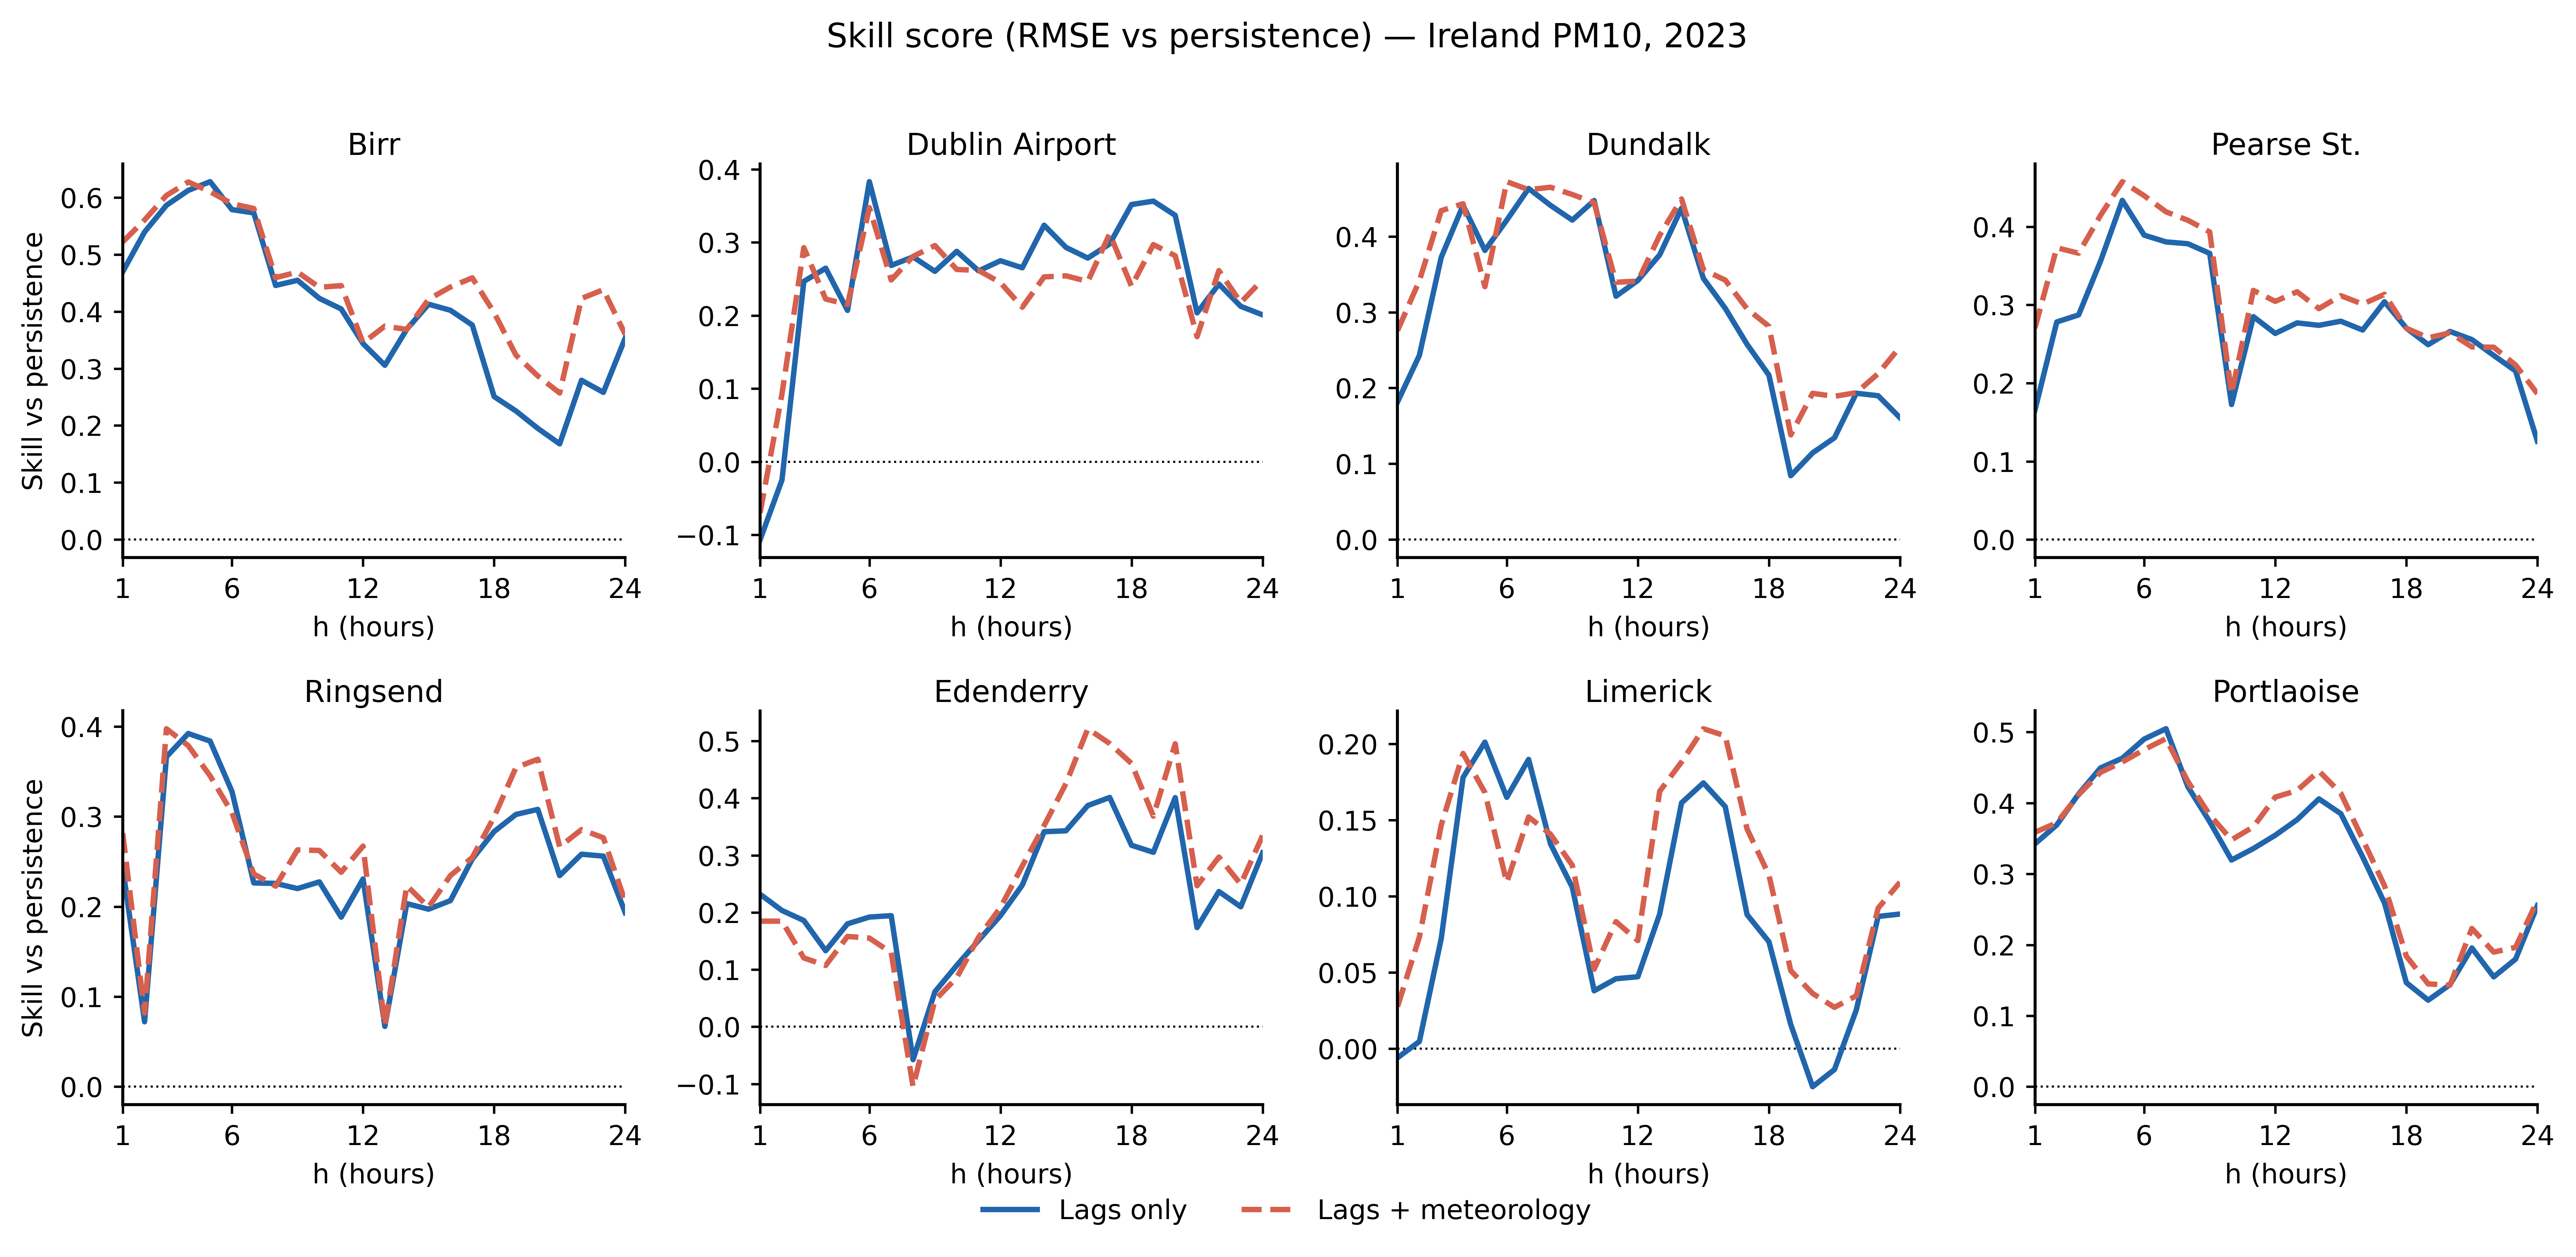
\includegraphics[width=0.98\textwidth]{serra_fig2_ireland_skill_by_station.png}
  \caption{Ireland (Jan--Jul 2023): persistence-relative RMSE skill
    $S_m(h)=1-\mathrm{RMSE}_m(h)/\mathrm{RMSE}_{\text{pers}}(h)$ over physical horizons
    $h=1,\ldots,24$~h for eight stations (one panel per station).  Blue solid:
    XGBoost (lags only).  Red dashed: XGBoost (lags + meteorology, using meteorological
    observations available at the forecast origin).  Horizontal line: $S=0$.
    Stations with $H^*_{\text{strict}}=24$ reach the 24-h evaluation boundary.}
  \label{fig:ireland_skill}
\end{figure*}

Table~\ref{tab:ireland_hstar} gives the corresponding station-level horizon
summaries. The contrast between Madrid and the Irish stations also shows why
an ``hour gained'' is not directly comparable across sites: the amount of
observable headroom depends on the underlying lags-only skill profile. This
makes inferential evidence for incremental meteorological information a
necessary complement to the descriptive horizon summaries.

\subsection{Descriptive gains do not scale to family-wise global support}

The paired loss-differential tests give a different view of the same
comparison. Under the primary dimensionally coherent overlap-based DM-HLN
specification ($q_{\text{overlap}}=0$), all 36 planned station--horizon tests
are valid (Table~\ref{tab:dm_q0}). Three comparisons have raw $p<0.05$, but
none survives global Bonferroni correction across the 36-test family (0/36).
At the narrower within-station level, Benjamini--Hochberg control retains
three signals: Birr at $h=1$, Madrid at $h=12$, and Pearse St.\ Dublin at
$h=6$. There is no contradiction between these findings. Local signals can
remain after within-station correction even when the planned family-wise
analysis yields no rejection, and the global 0/36 result should not be read
as evidence of equivalence or proof of no effect.

\subsection{Global conclusion remains unchanged under fixed automatic Newey--West sensitivity}

The overlap-based specification $q_{\text{overlap}}=0$ accounts for
dependence mechanically induced by forecast overlap under 24-h origin
spacing, but it does not rule out residual positive-lag dependence in the
loss differentials. We therefore repeat the analysis using the fixed
automatic Newey--West sensitivity reported in
Table~\ref{tab:dm_auto_nw}. The family-wise result does not change: no
comparison survives global Bonferroni correction (0/36). Three
within-station Benjamini--Hochberg signals again remain, although the set is
not identical. Birr at $h=1$ and Pearse St.\ Dublin at $h=6$ are retained
under both specifications. Madrid at $h=12$ appears only with the
overlap-based specification, whereas Pearse St.\ Dublin at $h=12$ appears
only with the automatic Newey--West sensitivity.

The global conclusion is therefore stable across the two audited dependence
specifications, while the small set of local signals is more sensitive to
that choice.

The complete cell-level inferential landscape is shown in
Figure~\ref{fig:dm_landscape}; the complete numerical results are provided
in Online Resource 1.

\begin{figure*}[t]
  \centering
  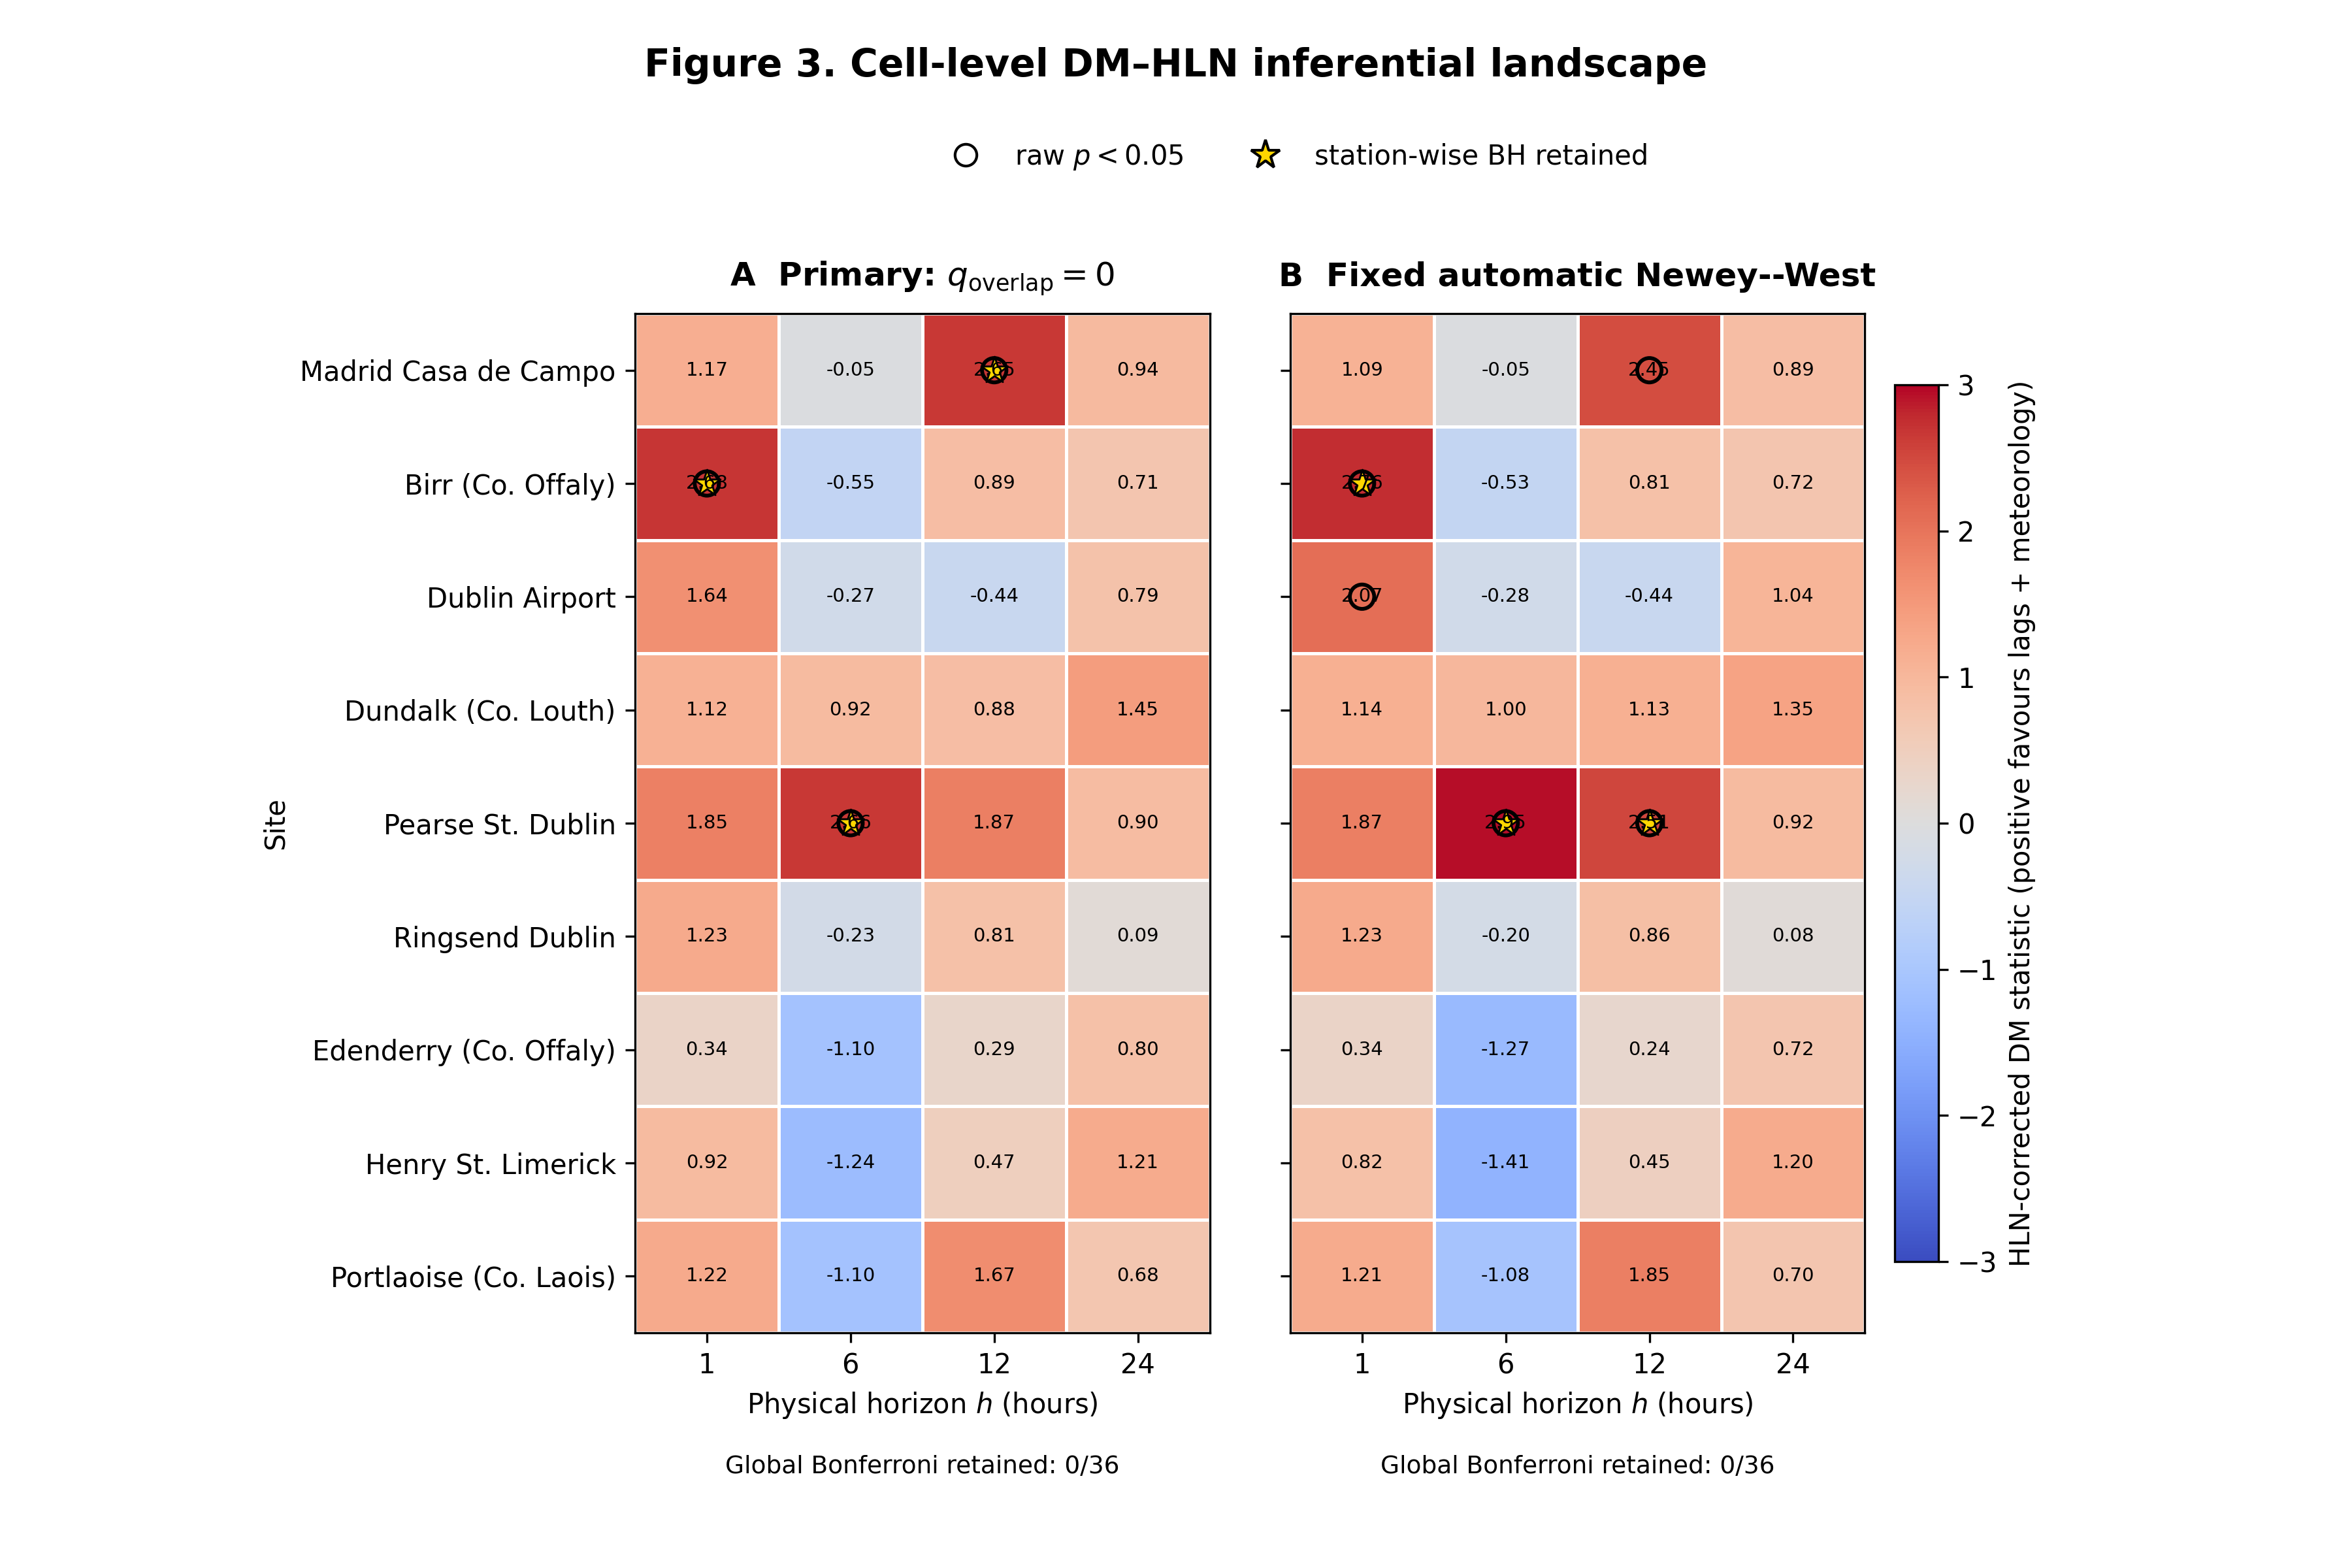
\includegraphics[width=0.98\textwidth]{serra_fig3_dm_inferential_landscape.png}
  \caption{Cell-level DM--HLN inferential landscape for the 36 planned
  site--horizon comparisons. Positive statistics favour the lags + meteorology
  information set, whereas negative statistics favour lags only. Both panels
  use the same symmetric colour scale. Open circles mark raw $p<0.05$ and
  stars mark station-wise Benjamini--Hochberg retention. No cell survives
  global Bonferroni correction (0/36); non-marked cells should not be
  interpreted as evidence of equivalence.}
  \label{fig:dm_landscape}
\end{figure*}

\section{Discussion}
\label{sec:discussion}
% ─────────────────────────────────────────────────────────────────────────────

Madrid illustrates why descriptive skill horizons are informative but not
sufficient for attribution. Adding meteorological observations extends the
strict positive-skill run from 9 to 17~h, a substantial change relative to
persistence. The relaxed measure, however, moves only from 15 to 17~h. Even
within one site, the apparent size of a ``horizon extension'' therefore
depends on whether the quantity of interest is continuity of positive skill
or the last horizon at which positive skill occurs.

Ireland exposes a different limitation of the same summary. Several lags-only
skill curves remain positive through most of the 24-h evaluation range, so
the strict descriptor often reaches $H_{\max}=24$ before meteorology is
added. The mean strict horizon increases only from 21.875 to 22.875~h
(+1.000~h), with five of eight lags-only cases already at the boundary and 11
station/condition cases reaching $H^*_{\text{strict}}=24$ overall. Small
changes in $H^*$ in this setting are therefore consistent with limited
observable headroom; they do not establish that meteorology contains no
incremental information.

The inferential analysis narrows the claim further. Under the primary
corrected DM-HLN specification ($q_{\text{overlap}}=0$), none of the 36
planned comparisons survives global Bonferroni correction, although a small
number of within-station Benjamini--Hochberg signals remain. Failure to obtain
family-wise rejection is not evidence of equivalence. It instead limits the
strength of the multi-site, multi-horizon claim that can be made about
attributing the descriptive gains to the added meteorological information.

Dependence in the loss-differential sequence is an important qualification.
The choice $q_{\text{overlap}}=0$ removes only the covariance mechanically
required by overlapping multi-step forecast errors; it does not imply
independence. The fixed automatic Newey--West sensitivity allows additional
positive-lag dependence without selecting the bandwidth from the observed
test outcomes. The global result remains 0/36 after Bonferroni correction,
while the identity of the limited local signals changes between
specifications. This stability at the family-wise level, combined with
instability in some local signals, argues against strong claims about
station-specific effects.

The evaluation design also has a practical statistical consequence. When
forecast origins and physical forecast horizons are expressed on different
time scales, the dependence parameters used for DM-HLN/HAC inference must be
defined in steps of the loss-differential sequence. Using the physical
horizon in hours directly would misrepresent the overlap structure when
origins are separated by 24~h.

Several limits determine the scope of these findings. The meteorological
covariates are observations available at forecast origin, not future NWP
forecasts. The 24-h evaluation range right-censors $H^*$ at several stations,
and the empirical evidence is limited to nine sites, the January--July 2023
evaluation window, and the XGBoost design considered here. The automatic
Newey--West analysis is a fixed sensitivity rather than an exhaustive model
of dependence, and the descriptive comparisons do not support causal
attribution. The main implication is therefore to keep three levels of
evidence separate: descriptive horizon extension, local inferential signals,
and family-wise global support for incremental information.

\section{Conclusions}
\label{sec:conclusions}
% ─────────────────────────────────────────────────────────────────────────────

The nine-site results show that descriptive horizon gains and inferential
attribution answer different questions. In Madrid, adding meteorological
observations extends the strict longest-contiguous positive-skill horizon
from 9 to 17~h, while the relaxed measure increases from 15 to 17~h. Across
the Irish network, changes are more heterogeneous and are often constrained
by the 24-h evaluation boundary.

The 36 planned, dimensionally corrected DM-HLN comparisons provide a more
restrictive inferential result. No comparison survives global Bonferroni
correction under either the overlap-based specification
($q_{\text{overlap}}=0$) or the fixed automatic Newey--West sensitivity.
That family-wise conclusion is stable across the two dependence
specifications, although the identities of the limited within-station BH
signals are not.

For multi-horizon environmental forecasting, a longer
persistence-relative skill horizon should therefore be interpreted first as
a descriptive result. Even a sizeable extension can coexist with limited
family-wise evidence that the added information set contributes incremental
predictability across the planned site--horizon family.

% ---------------------------------------------------------------------
% Full tables retained in the manuscript (no separate supplementary file)
% ---------------------------------------------------------------------
\FloatBarrier

\begin{table*}[!t]
\centering
\caption{Ireland station-level $H^*$ (hours) by model and criterion.
  $H^*_{\text{strict}}$ is the primary longest-contiguous positive-skill horizon;
  $H^*_{\text{relax}}$ is the secondary last-positive-skill horizon.  Entries of 24 for
  $H^*_{\text{strict}}$ indicate reaching the 24-h evaluation boundary ($H_{\max}=24$).}
\label{tab:ireland_hstar}
\small
\begin{adjustbox}{max width=0.96\textwidth}
\begin{tabular}{lrrrrrr}
\toprule
Station &
\multicolumn{2}{c}{XGBoost (lags only)} &
\multicolumn{2}{c}{XGBoost (lags + met.)} &
\multicolumn{2}{c}{SARIMA} \\
\cmidrule(lr){2-3}\cmidrule(lr){4-5}\cmidrule(lr){6-7}
& Strict & Relax & Strict & Relax & Strict & Relax \\
\midrule
Birr (Co.\ Offaly)      & 24 & 24 & 24 & 24 & 16 & 24 \\
Dublin Airport          & 22 & 24 & 23 & 24 & 24 & 24 \\
Dundalk (Co.\ Louth)    & 24 & 24 & 24 & 24 & 18 & 24 \\
Pearse St.\ Dublin      & 24 & 24 & 24 & 24 & 17 & 23 \\
Ringsend Dublin         & 24 & 24 & 24 & 24 &  9 & 20 \\
Edenderry (Co.\ Offaly) & 16 & 24 & 16 & 24 &  9 & 21 \\
Henry St.\ Limerick     & 17 & 24 & 24 & 24 &  4 & 17 \\
Portlaoise (Co.\ Laois) & 24 & 24 & 24 & 24 & 17 & 17 \\
\midrule
Mean                    & 21.875 & 24.0 & 22.875 & 24.0 & 14.3 & 21.3 \\
Mean $\Delta H^*_{\text{strict}}$ & \multicolumn{4}{c}{$+1.000$~h} & \multicolumn{2}{c}{---} \\
\bottomrule
\end{tabular}
\end{adjustbox}
\end{table*}

% T2 — Primary corrected overlap-based q_overlap = 0 DM-HLN inference (frozen results)
\begin{table}[t]
\centering
\small
\caption{Primary DM-HLN inference under the dimensionally coherent overlap-based specification.
Forecast origins are spaced by 24~h, so for physical horizons $h\in\{1,6,12,24\}$ the loss-differential horizon in sequence steps is $h_{\text{DM}}=\lceil h/24\rceil=1$ and the mechanically induced overlap bandwidth is $q_{\text{overlap}}=\max(0,h_{\text{DM}}-1)=0$ for all tests.  $q_{\text{overlap}}=0$ removes mechanically required overlap dependence but does not imply independence.
Global Bonferroni is applied across the 36 planned site--horizon tests; Benjamini--Hochberg (BH) is applied within each station (4 horizons) as a local sensitivity analysis.}
\label{tab:dm_q0}
\begin{tabular}{p{0.40\columnwidth}p{0.50\columnwidth}}
\toprule
Specification & Value \\
\midrule
Planned comparisons (sites $\times$ horizons) & $9\times 4 = 36$ \\
Valid tests & 36/36 \\
Raw $p<0.05$ & 3 \\
Global Bonferroni significant & 0/36 \\
Station-wise BH significant (count) & 3 \\
Station-wise BH identities & Birr ($h=1$); Madrid ($h=12$); Pearse St.\ Dublin ($h=6$) \\
\bottomrule
\end{tabular}
\end{table}

% T3 — Fixed automatic Newey--West HAC sensitivity (frozen results)
\begin{table}[t]
\centering
\small
\caption{Fixed automatic Newey--West sensitivity analysis for DM-HLN inference.
The HAC bandwidth is set by $q_{\text{auto}}=\lfloor 4\,(n/100)^{2/9}\rfloor$, allowing positive-lag autocovariances in the loss-differential sequence.  Global Bonferroni is applied across the 36 planned tests; BH is applied within each station (4 horizons) as a local sensitivity analysis.}
\label{tab:dm_auto_nw}
\begin{tabular}{p{0.40\columnwidth}p{0.50\columnwidth}}
\toprule
Specification & Value \\
\midrule
Planned comparisons (sites $\times$ horizons) & $9\times 4 = 36$ \\
Valid tests & 36/36 \\
Raw $p<0.05$ & 5 \\
Global Bonferroni significant & 0/36 \\
Station-wise BH significant (count) & 3 \\
Station-wise BH identities & Birr ($h=1$); Pearse St.\ Dublin ($h=6$); Pearse St.\ Dublin ($h=12$) \\
\bottomrule
\end{tabular}
\end{table}


\FloatBarrier

% Bibliography
% ─────────────────────────────────────────────────────────────────────────────
\bibliography{serra_references}


\FloatBarrier

\section*{Statements and Declarations}
% ─────────────────────────────────────────────────────────────────────────────

\subsection*{Funding}
No funds, grants, or other support were received for conducting this study or
preparing this manuscript.

\subsection*{Competing interests}
The author has no relevant financial or non-financial interests to disclose.

\subsection*{Author contributions}
The author conceived the study, designed the methodology, performed the analyses, developed the software, interpreted the results, and wrote and approved the manuscript.

\subsection*{Data availability}
The public GitHub repository \url{https://github.com/fedeg-umh-es/P1_PM10_Meteorology_Hstar}
contains the versioned analysis code, the processed and regenerated study
artifacts archived there, figure-generation support, run metadata, and the
final overlap-based and automatic Newey--West inferential tables reported in
this manuscript for the underlying meteorology experiment.
The Irish station evaluations were regenerated from recovered source datasets
using the versioned analysis pipeline. The row-level predictions from the
originally executed Irish computational run were not retained; therefore, the
reported Irish results correspond to the documented regeneration rather than
recovery of the original prediction files. Raw source data are available from
the Madrid City Council and the Irish Environmental Protection Agency under
their respective open-data terms.

\subsection*{Ethics approval and consent to participate}
Not applicable. The study used environmental monitoring data and involved no
human participants or animals.

\subsection*{Consent for publication}
Not applicable.

\subsection*{Acknowledgements}
The author thanks the Madrid City Council and the Irish Environmental Protection
Agency for providing open-access air-quality and meteorological data.



\FloatBarrier

% ─────────────────────────────────────────────────────────────────────────────

\end{document}
